\section{Teilversuch 1: Bestimmung der Schallgeschwindigkeit in Luft}
	\subsection{Bestimmung der Wellenlänge}
		Um die Wellenlänge zu bestimmen, war es in der Fragestellung der Auswertung verlangt, eine optimale Kurve durch die Messpunkte zu legen. Statt Millimeterpapier wird aber in diesem Fall \gnuplot{} benutzt. Das Prozess der Wellenlängebestimmung wird dann ein bisschen anders aussehen.

		Laut Theorie lässt eine Welle mittels einer Sinus bzw. Cosinus Funktion beschreiben. Die Summe von zwei solchen Wellen liefert dann noch eine Sinus bzw. Cosinus Funktion. Da wir aber nur die Lautstärke mittels Mikrofonspannung messen können, entsprechen die Messwerte die absolute Betrag von dieser Funktion. Im Allgemein, lässt die Messwerte durch die folgende Funktion beschreiben:
		\begin{equation}
			U_\text{eff} = \abs{A\sin\left[kx - h\right]} + c = \abs{A\sin\left[\frac{2\pi}{\lambda}(x - b)\right]} + c
		\end{equation}
		wobei $\lambda =$ Wellenlänge und $\mathbb{R} \ni b, c = $ konstante. 

		Als physikalische Bedeutung ist $c$ die Raumhintergrund, $b$ die Position des ersten Minimums und $A$ die maximale Mikrofonspannung ohne die Raumhintergrund. 

		\newpage
		\textbf{1. Messreihe}\\
		Fehler bei Messung der Spannung $\Delta U_\text{eff} = \SI{0.1}{\milli\volt}$ \\
		Fehler bei Messung der Position $\Delta x = \SI{0.5}{\milli\meter}$ 

		\begin{center}
			\begin{tabular}{l *{10}{r}}
				\toprule
				$n$ & $1$ & $2$ & $3$ & $4$ & $5$ & $6$ & $7$ & $8$ & $9$ & $10$  \\
				\midrule
				$x/\si{\milli\meter}$ & \num{63.5} & \num{70.0} & \num{80.0} & \num{90.0} & \num{100.0} & \num{110.0} & \num{120.0} & \num{130.0} & \num{140.0} & \num{150.0}  \\
				$U_\text{eff} / \si{\milli\volt}$ & \num{42.9} & \num{40.3} & \num{27.9} & \num{9.4} & \num{12.8} & \num{31.0} & \num{42.2} & \num{45.1} & \num{39.7} & \num{26.2}  \\
				\bottomrule
				\toprule
				$n$ & $11$ & $12$ & $13$ & $14$ & $15$ & $16$ & $17$ & $18$ & $19$ & $20$ \\
				\midrule
				$x/\si{\milli\meter}$ & \num{160.0} & \num{170.0} & \num{180.0} & \num{190.0} & \num{200.0} & \num{210.0} & \num{220.0} & \num{230.0} & \num{240.0} & \num{250.0} \\
				$U_\text{eff} / \si{\milli\volt}$  & \num{7.0} & \num{15.5} & \num{33.2} & \num{42.6} & \num{44.1} & \num{36.4} & \num{21.0} & \num{2.0} & \num{20.7} & \num{36.3}  \\
				\bottomrule
				\toprule
				$n$ & $21$ & $22$ & $23$ & &&&&&& \\
				\midrule
				$x/\si{\milli\meter}$ & \num{260.0} & \num{270.0} & \num{280.0} & &&&&&& \\
				$U_\text{eff} / \si{\milli\volt}$ & \num{44.2} & \num{43.1} & \num{33.3} & &&&&&& \\
				\bottomrule 
			\end{tabular}
		\end{center}

		\textbf{2. Messreihe bei erstem und letztem Minimum}\\
		Fehler bei Messung der Spannung $\Delta U_\text{eff} = \SI{0.2}{\milli\volt}$ \\
		Fehler bei Messung der Position $\Delta x = \SI{0.5}{\milli\meter}$

		\begin{center}
			\begin{tabular}{l *{4}{r} | rr}
				\toprule
				$U_\text{eff} / \si{\milli\volt}$ & $x_1 / \si{\milli\meter}$ & $x_2 / \si{\milli\meter}$ & $x_3 / \si{\milli\meter}$ & $x_4 / \si{\milli\meter}$ & $x_{1,2} / \si{\milli\meter}$ & $x_{3,4} / \si{\milli\meter}$ \\
				\midrule
				\num{5.0} & \num{93.5} & \num{97.0} & \num{232.0} & \num{228.0}   & \num{95,3} & \num{230,0} \\
				\num{10.0} & \num{98.5} & \num{89.5} & \num{225.5} & \num{234.5}  & \num{94,0} & \num{230,0} \\
				\num{15.0} & \num{89.0} & \num{102.0} & \num{237.5} & \num{223.0} & \num{95,5} & \num{230,3} \\
				\num{20.0} & \num{104.5} & \num{84.5} & \num{220.0} & \num{237.5} & \num{94,5} & \num{228,8} \\
				\num{25.0} & \num{87.5} & \num{107.0} & \num{242.0} & \num{217.5} & \num{97,3} & \num{229,8} \\
				\bottomrule
			\end{tabular}
		\end{center}
		Die Mittelwerte $x_{1,2} = (x_1 + x_2)/2$ bzw. $x_{3,4} = (x_3 + x_4)/2$ haben als Fehler:
		\begin{equation}
			\Delta x_{1,2} = \Delta x_{3,4} = \frac{\SI{0.5}{\milli\meter}}{\sqrt{2}} = \SI{0,4}{\milli\meter}
		\end{equation}
		Wenn wir die erste Reihe betrachten, können wir das erste Minimum bei $x = (\SI{93,5}{\milli\meter} + \SI{97,0}{\milli\meter})/2 = \SI{95.25}{\milli\meter}$ und das letzte Minimum bei $x = (\SI{232.0}{\milli\meter} + \SI{228.0}{\milli\meter})/2 = \SI{230.0}{\milli\meter}$ einschätzen. Die Wellenlänge ist dann ungefähr $\SI{230}{\milli\meter} - \SI{95.25}{\milli\meter} = \SI{134.75}{\milli\meter}$. 

		Da es bei ungefähr $x = \SI{230.0}{\milli\meter}$ ein Minimum liegt, ist der Messwert für $n = 18$ mit $U_\text{eff} = \SI{2.0}{\milli\volt}$ ungefähr der Raumhintergrund. 

		Der größte Messwert liegt bei $n = 21$ mit $U_\text{eff} = \SI{44.2}{\milli\volt}$. Dieser Wert wird dann als ein Maximumwert geschätzt.

		Wir benutzen deshalb die folgende Werte als Anfangseinschätzungen bei der Kurveanpassung:
		\begin{center}
			\begin{tabular}{l r}
				\toprule
				Variable & Wert \\
				\midrule
				$A$ & \num{45} \\
				$\lambda$ & \num{134.75} \\
				$b$ & \num{95.2} \\
				$c$ & \num{2} \\
				\bottomrule
			\end{tabular}
		\end{center}

		Die Daten wurden dann mit \gnuplot{} geplottet und es wurde eine Kurvenanpassung durchgeführt. Der Punkt bei $(87,5, 25,0)$ ist aber zu weit von der Kurve abgeweicht und wird als Anomalie vernachlässigt. Alle nötige Rechnungen erfolgt im \gnuplot{}. Siehe Appendix \ref{appdx:gnuplotTV1} für die genauere Rechnungen.

		Normale Anpassungsalgorithmen (Methode der kleinsten Quadrate) setzen voraus, dass die $x$-Variable die unabhängige Variable ist und als fehlerfrei genommen werden kann. Da es sich bei diesem Versuch um zwei gemessene Variablen handelt, gibt es bei beiden Variablen $y = U_\text{eff}$ und $x$ Fehler. Die Fehler müssen dann während der Kurvenanpassung berücksichtigt werden. 

		\begin{figure}[H]
			\centering
			% GNUPLOT: LaTeX picture with Postscript
\begingroup
  \makeatletter
  \providecommand\color[2][]{%
    \GenericError{(gnuplot) \space\space\space\@spaces}{%
      Package color not loaded in conjunction with
      terminal option `colourtext'%
    }{See the gnuplot documentation for explanation.%
    }{Either use 'blacktext' in gnuplot or load the package
      color.sty in LaTeX.}%
    \renewcommand\color[2][]{}%
  }%
  \providecommand\includegraphics[2][]{%
    \GenericError{(gnuplot) \space\space\space\@spaces}{%
      Package graphicx or graphics not loaded%
    }{See the gnuplot documentation for explanation.%
    }{The gnuplot epslatex terminal needs graphicx.sty or graphics.sty.}%
    \renewcommand\includegraphics[2][]{}%
  }%
  \providecommand\rotatebox[2]{#2}%
  \@ifundefined{ifGPcolor}{%
    \newif\ifGPcolor
    \GPcolortrue
  }{}%
  \@ifundefined{ifGPblacktext}{%
    \newif\ifGPblacktext
    \GPblacktexttrue
  }{}%
  % define a \g@addto@macro without @ in the name:
  \let\gplgaddtomacro\g@addto@macro
  % define empty templates for all commands taking text:
  \gdef\gplbacktext{}%
  \gdef\gplfronttext{}%
  \makeatother
  \ifGPblacktext
    % no textcolor at all
    \def\colorrgb#1{}%
    \def\colorgray#1{}%
  \else
    % gray or color?
    \ifGPcolor
      \def\colorrgb#1{\color[rgb]{#1}}%
      \def\colorgray#1{\color[gray]{#1}}%
      \expandafter\def\csname LTw\endcsname{\color{white}}%
      \expandafter\def\csname LTb\endcsname{\color{black}}%
      \expandafter\def\csname LTa\endcsname{\color{black}}%
      \expandafter\def\csname LT0\endcsname{\color[rgb]{1,0,0}}%
      \expandafter\def\csname LT1\endcsname{\color[rgb]{0,1,0}}%
      \expandafter\def\csname LT2\endcsname{\color[rgb]{0,0,1}}%
      \expandafter\def\csname LT3\endcsname{\color[rgb]{1,0,1}}%
      \expandafter\def\csname LT4\endcsname{\color[rgb]{0,1,1}}%
      \expandafter\def\csname LT5\endcsname{\color[rgb]{1,1,0}}%
      \expandafter\def\csname LT6\endcsname{\color[rgb]{0,0,0}}%
      \expandafter\def\csname LT7\endcsname{\color[rgb]{1,0.3,0}}%
      \expandafter\def\csname LT8\endcsname{\color[rgb]{0.5,0.5,0.5}}%
    \else
      % gray
      \def\colorrgb#1{\color{black}}%
      \def\colorgray#1{\color[gray]{#1}}%
      \expandafter\def\csname LTw\endcsname{\color{white}}%
      \expandafter\def\csname LTb\endcsname{\color{black}}%
      \expandafter\def\csname LTa\endcsname{\color{black}}%
      \expandafter\def\csname LT0\endcsname{\color{black}}%
      \expandafter\def\csname LT1\endcsname{\color{black}}%
      \expandafter\def\csname LT2\endcsname{\color{black}}%
      \expandafter\def\csname LT3\endcsname{\color{black}}%
      \expandafter\def\csname LT4\endcsname{\color{black}}%
      \expandafter\def\csname LT5\endcsname{\color{black}}%
      \expandafter\def\csname LT6\endcsname{\color{black}}%
      \expandafter\def\csname LT7\endcsname{\color{black}}%
      \expandafter\def\csname LT8\endcsname{\color{black}}%
    \fi
  \fi
    \setlength{\unitlength}{0.0500bp}%
    \ifx\gptboxheight\undefined%
      \newlength{\gptboxheight}%
      \newlength{\gptboxwidth}%
      \newsavebox{\gptboxtext}%
    \fi%
    \setlength{\fboxrule}{0.5pt}%
    \setlength{\fboxsep}{1pt}%
\begin{picture}(8640.00,5760.00)%
    \gplgaddtomacro\gplbacktext{%
      \csname LTb\endcsname%%
      \put(682,704){\makebox(0,0)[r]{\strut{}$0$}}%
      \put(682,1489){\makebox(0,0)[r]{\strut{}$10$}}%
      \put(682,2274){\makebox(0,0)[r]{\strut{}$20$}}%
      \put(682,3058){\makebox(0,0)[r]{\strut{}$30$}}%
      \put(682,3843){\makebox(0,0)[r]{\strut{}$40$}}%
      \put(682,4628){\makebox(0,0)[r]{\strut{}$50$}}%
      \put(814,484){\makebox(0,0){\strut{}$50$}}%
      \put(2300,484){\makebox(0,0){\strut{}$100$}}%
      \put(3786,484){\makebox(0,0){\strut{}$150$}}%
      \put(5271,484){\makebox(0,0){\strut{}$200$}}%
      \put(6757,484){\makebox(0,0){\strut{}$250$}}%
      \put(8243,484){\makebox(0,0){\strut{}$300$}}%
      \csname LTb\endcsname%%
      \put(1854,2823){\makebox(0,0)[l]{\strut{}\textcolor{red}{\scriptsize Anomalie}}}%
    }%
    \gplgaddtomacro\gplfronttext{%
      \csname LTb\endcsname%%
      \put(209,2901){\rotatebox{-270}{\makebox(0,0){\strut{}Mikrofonspannung $U_\text{eff}$ ($\si{\milli\volt}$)}}}%
      \put(4528,154){\makebox(0,0){\strut{}Position auf optischen Schiene $x$ ($\si{\milli\meter}$)}}%
      \put(4528,5429){\makebox(0,0){\strut{}Mikrofonspannung als Funktion der Position}}%
      \csname LTb\endcsname%%
      \put(7256,4838){\makebox(0,0)[r]{\strut{}$\abs{43,06084\sin\left[\frac{2\pi}{135,63770}\left(x - 94,40624\right)\right]} + 1,62297$}}%
      \csname LTb\endcsname%%
      \put(7256,4442){\makebox(0,0)[r]{\strut{}Messpunkte}}%
    }%
    \gplbacktext
    \put(0,0){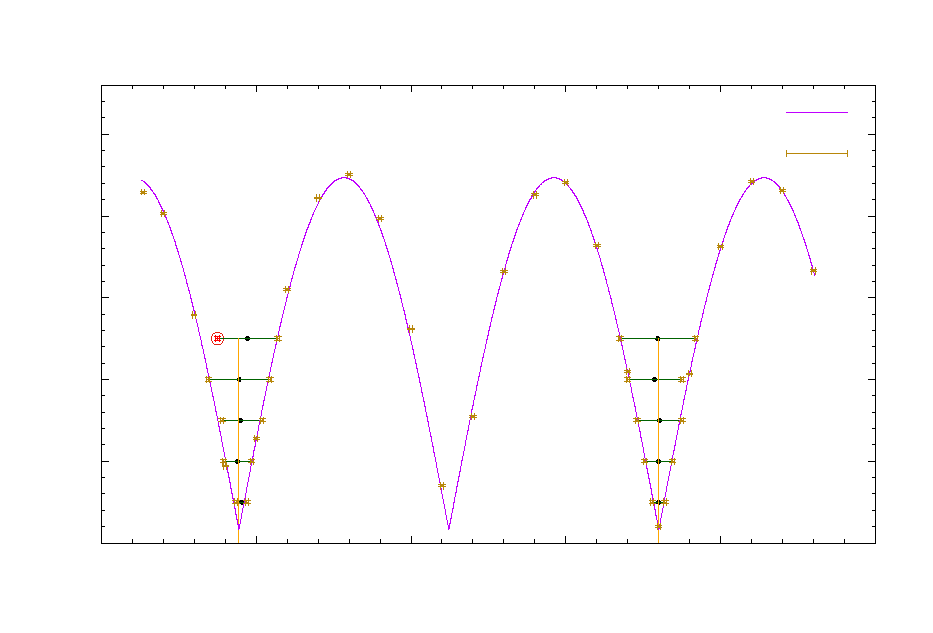
\includegraphics{tv1-plot}}%
    \gplfronttext
  \end{picture}%
\endgroup

			\caption{\centering Messung der Mikrofonspannung bei verschiedenen Orten \captionbr $\chi^2_{\text{red}} = \num{3.7408} > 1 \implies$ Nicht so gute Anpassung}
			\label{fig:tvone-plot}
			\vspace{-1em}
		\end{figure}
		Das wenig ideale $\chi^2_{\text{red}}$ lässt sich dadurch erklären, dass die Fehler wahrscheinlich wesentlich unterschätzt wurden. 

		Als Endergebnis haben wir:
		\begin{center}
			\begin{tabular}{l r r}
				\toprule
				Variable & Rohausgabe & Gerundet \\
				\midrule
				$A$ & \SI{43.0608(5247)}{\milli\volt} & \SI{43.1(6)}{\milli\volt} \\
				$\lambda$ & \SI{135.6377(3153)}{\milli\meter} & \SI{135.6(4)}{\milli\meter} \\
				$b$ & \SI{94.4062(2371)}{\milli\meter} & \SI{94.41(24)}{\milli\meter} \\
				$c$ & \SI{1.6230(4747)}{\milli\volt}  & \SI{1.6(5)}{\milli\volt} \\
				\bottomrule
			\end{tabular}
		\end{center}

		Von der angepassten Kurve weichen die Werte aus der zweiten Messreihe durchschnittlich mehr als die Werte aus der ersten Messreihe ab. Diese Punkten sind mit grünen Linien angezeichnet. Diese Abweichung kann darauf zurückgeführt werden, dass wir bei dieser Messung auf der schwankende Mikrofonspannung während der ungenauen Verschiebung des Mikrofons aufpassen müssen. Das kann zu einen Fehler führen, der deutlich größer als was wir hier geschätzt haben. 

		Wir rechnen rückwärts und leiten die beiden Ausgleichsgerade von der angepassten Kurve her. Die schwarzen Punkte auf der grünen Linien sind die Mittelpunkte der zur Abszisse parallelen Strecken. Die linke orange Linie ist gegeben durch $x_e = b$ und die rechte $x_l = b + \lambda$, wobei $b$ und $\lambda$ aus der Kurvenanpassung kommt. Explizit geschrieben:
		\begin{align}
			x_e & = \SI{94.41(24)}{\milli\meter},\\
			x_l & = \SI{94.41(24)}{\milli\meter} + \SI{135.6(4)}{\milli\meter} = \SI{230,0(5)}{\milli\meter} \label{eqn:xl}
		\end{align}
		wobei der Fehler in Gleichung \eqref{eqn:xl} durch $\Delta x_l = \sqrt{\pbrace{\SI{0,24}{\milli\meter}}^2 + \pbrace{\SI{0,4}{\milli\meter}}^2} = \SI{0,5}{\milli\meter}$ gegeben ist. 

		Wir vergleichen jetzt diese Werte mit dem Mittelwert und Standardabweichung von $x_{1,2}$ und $x_{3,4}$. Der Wert von $x_{1,2}$ bei Spannung $U_\text{eff} = \SI{25,0}{\milli\volt}$ wird vernachlässigt. Die Standardabweichung ist hier wegen der Schwerigkeit der Schätzung aus geplotteten Graph statt grob Betrachtung der Zeichnung benutzt. Mithilfe eines Python Skript (Appendix \ref{appdx:pythontv1}) bekommen wir die folgenden Werte:
		\begin{center}
			\begin{tabular}{lr}
				\toprule
				$x_e = x_{1,2}$ & \SI{94,8(7)}{\milli\meter} \\
				$x_l = x_{3,4}$ & \SI{229,8(6)}{\milli\meter} \\
				\bottomrule
			\end{tabular}
		\end{center}
		Die Werte stimmen miteinander überein. Es ist anschaulich, dass die orange Linien gute Annäherungen für beide Reihe von Mittelpunkten sind. Wir benutzen nun die Wellenlänge aus der Kurvenanpassung:
		\begin{equation}
			\lambda = \SI{135.6(4)}{\milli\meter}
		\end{equation}

	\subsection{Bestimmung der Schallgeschwindigkeit in Luft}
		Die Schallgeschwindigkeit $v$ und Wellenlänge $\lambda$ haben den folgenden Zusammenhang:
		\begin{align}
			v &= f\lambda \\
			\implies \Delta v &= \gausserror{v}{f, \lambda} = \sqrt{\pbrace{\lambda\Delta f}^2 + \pbrace{f\Delta \lambda}^2}
		\end{align}
		Mit der folgenden Werten:
	    \begin{center}
	        \begin{tabular}{lrl}
	            \toprule
	            Variable & Wert & Bedeutung \\
	            \midrule
	            $f$ & \SI{2,54(1)}{\kilo\hertz} & Frequenz \\
	            $\lambda$ & \SI{135.6(4)}{\milli\meter} & Wellenlänge \\
	            \bottomrule
	        \end{tabular}
	    \end{center}
	    lässt sich $v$ und $\Delta v$ bestimmen:
	    \begin{align}
			v &= \pbrace{\SI{2,54e3}{\hertz}}\pbrace{\SI{135,6e-3}{\meter}} = \SI{344,424}{\meter\per\second} \\
			\implies \Delta v &= \sqrt{\pbrace{\pbrace{\SI{135,6e-3}{\meter}}\pbrace{\SI{0,01e3}{\hertz}}}^2 + \pbrace{\pbrace{\SI{2,54e3}{\hertz}} \pbrace{\SI{0,4e-3}{\meter}}}^2} \notag \\ 
			&=  \SI{1,694}{\meter\per\second} \sigfig{4}
		\end{align}
		Daraus folgt, $v = \SI{344,4(17)}{\meter\per\second}$

		Aus der Anleitung ist der Schallgeschwindigkeit $v$ proportional zur $\sqrt{T}$, wobei $T$ die absolute Temperatur ist. Mit $T = \pbrace{\pbrace{\num{21,0(1)}} + 273.15} \si{\kelvin} = \SI{294.15(10)}{\kelvin} = \SI{294.2(1)}{\kelvin}$ lässt sich eine theoretische Schallgeschwindigkeit berechnen:
		\begin{align}
			v &= v_0\cdot\sqrt{\frac{T}{T_0}} = \pbrace{\SI{331}{\meter\per\second}}\cdot\sqrt{\frac{\SI{294,15}{\kelvin}}{\SI{273,15}{\kelvin}}} = \SI{343,488}{\meter\per\second} \sigfig{6} \\
			\Delta v &= \gausserror{v}{T} = \frac{v_0}{\sqrt{T_0}}\cdot\frac{1}{2}\cdot\frac{1}{\sqrt{T}}\pbrace{\Delta T} = \frac{v_0}{2\sqrt{T\cdot T_0}} \pbrace{\Delta T} \notag \\
			&= \frac{\SI{331}{\meter\per\second}}{2\sqrt{\pbrace{\SI{294,15}{\kelvin}}\pbrace{\SI{273,15}{\kelvin}}}} \pbrace{\SI{0,1}{\kelvin}} \notag \\
			&= \SI{0,0584}{\meter\per\second} \sigfig{3}
		\end{align}
		wobei $v_0$ und $T_0$ jeweils die Schallgeschwindigkeit und die absolute Temperatur bei $\SI{0}{\celsius}$ sind. Genauere Werte sind hier benutzt, um mögliche Rundungsfehler zu vermeiden. 

		Daraus folgt, $v_\text{th} = \SI{343,49(6)}{\meter\per\second}$

		Im Vergleich erhalten wir:
		\begin{center}
	        \begin{tabular}{lr}
	            \toprule
	            $v_\text{exp}$ & \SI{344,4(17)}{\meter\per\second} \\
	            $v_\text{th}$ & \SI{343,49(6)}{\meter\per\second} \\
	            \bottomrule
	        \end{tabular}
	    \end{center}
	    Der theoretische Wert $v_\text{th}$ liegt im Fehlerintervall des experimentellen Wertes. Die Werte stimmen also miteinander überein.

	\subsection{Bestimmung des Adiabatenexponentes $\gamma$ der Luft}
		Aus der Anleitung ist der Adiabatenexponent $\gamma$ und folglich der dazugehörige Fehler $\Delta \gamma$ gegeben durch:
		\begin{align}
			v &= f \lambda = \sqrt{\gamma \frac{RT}{M}}  \iff \gamma = \pbrace{\frac{M}{R}}\cdot\frac{f^2\lambda^2}{T} = \pbrace{\frac{M}{R}}\cdot\frac{f^2\lambda^2}{\theta + \SI{273.15}{\kelvin}}  \\
			\Delta \gamma &= \gausserror{\gamma}{f, \lambda, T} \notag \\
			\text{\scriptsize (AMW)} &= \frac{Mf^2\lambda^2}{RT} \sqrt{\pbrace{\frac{\Delta T}{T}}^2 + \pbrace{\frac{2\Delta f}{f}}^2 + \pbrace{\frac{2\Delta \lambda}{\lambda}}^2} \notag \\
			&= \frac{Mf^2\lambda^2}{R\pbrace{\theta + \SI{273.15}{\kelvin}}} \sqrt{\pbrace{\frac{\Delta \theta}{\theta + \SI{273.15}{\kelvin}}}^2 + \pbrace{\frac{2\Delta f}{f}}^2 + \pbrace{\frac{2\Delta \lambda}{\lambda}}^2}
		\end{align}
		Mit der folgenden Werten:
	    \begin{center}
	        \begin{tabular}{lrl}
	            \toprule
	            Variable & Wert & Bedeutung \\
	            \midrule
	            $M$ & \SI{28,96}{\gram\per\mol} & Molare Masse von trockener Luft \\
	            $R$ & \SI{8.314463}{\kilo\gram\meter\squared\per\kelvin\per\mol\per\second\squared} & Allgemeine Gaskonstante (CODATA 2018) \\
	            $f$ & \SI{2,54(1)}{\kilo\hertz} & Frequenz \\
	            $\lambda$ & \SI{135.6(4)}{\milli\meter} & Wellenlänge \\
	            $\theta$ & \SI{21,0(1)}{\celsius} & Temperatur der Luft im Labor \\
	            \bottomrule
	        \end{tabular}
	    \end{center}
	    lässt sich $\gamma$ und $\Delta \gamma$ bestimmen:
	    \begin{align}
	    	\gamma &= \pbrace{\frac{\num{28,96e-3}}{\num{8.314463}}\si{\kelvin\second\squared\per\meter\squared}}\cdot\frac{\pbrace{\SI{2,54e3}{\hertz}}^2\pbrace{\SI{135.6e-3}{\meter}}^2}{\pbrace{\num{21,0} + \num{273.15}}\si{\kelvin}} \notag \\
	    	&= \num{1,40470} \sigfig{6} \\
	    	\Delta\gamma &= \pbrace{\frac{\num{28,96e-3}}{\num{8.314463}}\si{\kelvin\second\squared\per\meter\squared}}\cdot\frac{\pbrace{\SI{2,54e3}{\hertz}}^2\pbrace{\SI{135.6e-3}{\meter}}^2}{\pbrace{\num{21,0} + \num{273.15}}\si{\kelvin}} \notag \\
	    	&~~~~~\times \sqrt{\pbrace{\frac{\SI{0.1}{\kelvin}}{\pbrace{\num{21,0} + \num{273.15}}\si{\kelvin}}}^2 + \pbrace{\frac{2\cdot\SI{0,01}{\kilo\hertz}}{\SI{2,54}{\kilo\hertz}}}^2 + \pbrace{\frac{2\cdot\SI{0,4}{\milli\meter}}{\SI{135.6}{\milli\meter}}}^2} \notag \\
	    	&= \num{0,0138} \sigfig{3}
		\end{align}
		Daraus folgt, $\gamma = \num{1,405(14)}$. $\gamma$ ist einheitslos.

		Im Abschnitt 1.5 der Anleitung wurde der theoretische Wert von $\gamma$ als $\num{1.4}$ genannt. Dieser Wert liegt in dem Fehlerintervall des experimentellen Wertes. Die Werte stimmen also miteinander überein.